\chapter{Quadratic Form}\label{Quadratic Form}
% chktex-file 31
\section{Quadratic Form Fundamentals}\label{Quadratic Form Fundamentals}
\begin{itemize}
  \item \dd{Quadratic form}: a polynomial with terms all of \emph{degree two}.
    \begin{itemize}
      \item The quadratic form is central to various fields of mathematics, and not to be confused with quadratic equation.
      \item The quadratic form is one case of a more general concept of homogenous polynomials (not covered here).
    \end{itemize}
  \item Note: let \tbm{S} denote a square matrix going forward, however, such matrices will not necessarily be symmetric or invertible.
  \subsection{Quadratic Form in Algebra}\label{Quadratic Form in Algebra}
  \begin{itemize}
    \item \dd{Quadratic form}: essentially the \amp{``energy \(\epsilon\)''} in a matrix \ttt{\tbm{S}} over a coordinate space defined by a vector \(\str{\bm{w}}\), i.e.,
    \[%%%%%%%%%%%%%%%%%%%%%%%%%%%%%%%%%%%%%%%%%%%%%%%
    \underbrace{\bm{\str{w}}^T}_{1 \times \str{n} }
    \underbrace{\bm{\ttt{S}}}_{\str{n} \times \str{n} }
    \underbrace{\bm{\str{w}}}_{\str{n} \times 1} = \amp{\epsilon}
    \]%%%%%%%%%%%%%%%%%%%%%%%%%%%%%%%%%%%%%%%%%%%%%%%
    \item Generalized, if \ttt{\(\bm{S}=
    \begin{bmatrix}
    a & b \\
    c & d 
    \end{bmatrix}\)} and \str{\(\bm{w}=\begin{bmatrix} x \\ y \end{bmatrix}\)}, then a quadratic form becomes more apparent, i.e.,
    \[%%%%%%%%%%%%%%%%%%%%%%%%%%%%%%%%%%%%%%%%%%%%%%%
    \str{\bm{w}}^T \ttt{\bm{S}} \str{\bm{w}} = \ttt{a}\str{x}^2 + (\ttt{b}+\ttt{c})\str{xy} + \ttt{d}\str{y}^2 = \amp{\epsilon}
    \]%%%%%%%%%%%%%%%%%%%%%%%%%%%%%%%%%%%%%%%%%%%%%%%
    \item The features of coefficients described in \(\ttt{\bm{S}}\) determine the \hyperref[Definiteness]{\dlink{definiteness}} of a matrix, which will be covered later in this chapter.
    \item If \(\ttt{\bm{S}}\) is symmetric, then the transpose of the quadratic form is equivalent to the original form, i.e.,
    \[%%%%%%%%%%%%%%%%%%%%%%%%%%%%%%%%%%%%%%%%%%%%%%%
    \str{\bm{w}}^T \ttt{\bm{S}} \str{\bm{w}} =  \str{\bm{w}}^{T} \ttt{\bm{S}}^T \str{\bm{w}}^{TT} =  \str{\bm{w}}^T \ttt{\bm{S}} \str{\bm{w}}
    \]%%%%%%%%%%%%%%%%%%%%%%%%%%%%%%%%%%%%%%%%%%%%%%%
    \begin{itemize}
      \item Sometimes this property is part of the definition of the quadratic form, and thus requires matrix \ttt{\tbm{S}} to be square and symmetric, yielding a polynomial with a slightly simpler form, e.g., \(\ttt{2b}\str{\bm{xy}}\) vs. \((\ttt{b}+\ttt{c})\str{xy}\)
    \end{itemize}
    \item The quadratic form works for any dimension, as long \(\ttt{\bm{S}}\) is square and \(\str{\bm{w}}\) has the same number of elements as size of \(\ttt{\bm{S}}\), and always yields a single number \(\amp{\epsilon}\)
  \end{itemize}
  
  \subsection{Quadratic Form in Geometry}\label{Quadratic Form in Geometry}
  \begin{itemize}
    \item The quadratic form can also be thought of a function that takes a matrix with a distinct vector as inputs, i.e.,
    \[%%%%%%%%%%%%%%%%%%%%%%%%%%%%%%%%%%%%%%%%%%%%%%%
    f(\ttt{\bm{S}},\str{\bm{w}}_{i,\, j}) = \amp{\epsilon}
    \]%%%%%%%%%%%%%%%%%%%%%%%%%%%%%%%%%%%%%%%%%%%%%%%
    \item Iterating over all distinct values of \(i, j\) over field yields numerous values of \(\amp{\epsilon}\), indicating the \amp{``energy''} on the z-axis, the resulting \emph{surface} of the matrix given the coordinate space is thus defined by \(\str{\bm{w}}\).
    \item Changing the elements in \(\ttt{\bm{S}}\) changes the shape of the matrix and thus the space it defines; keeping \(\str{\bm{w}}\) constant, but altering \(\ttt{\bm{S}}\), yields different surface shapes based on values of \(\amp{\epsilon}\) as values of \(i, j\) are iterated over the coordinate plane.
    \item Below are the most basic quadratic forms in space, each representing different \hyperref[Definiteness]{\dlink{ definiteness}} of real matrices.
    \medskip
    \begin{center}
      \scalebox{0.69}{
        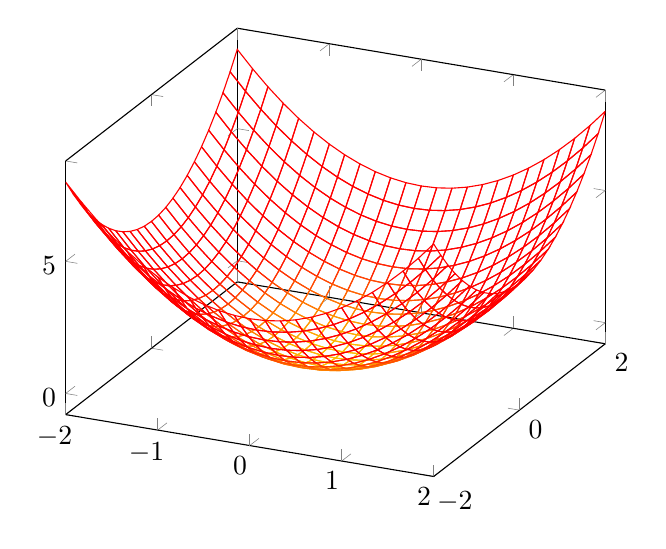
\begin{tikzpicture}
        \begin{axis}[samples=25]
        \addplot3[surf,mesh, point meta min=-2, point meta max=2, domain=-2:2] {x^2+y^2};
        \end{axis}
        \end{tikzpicture}
        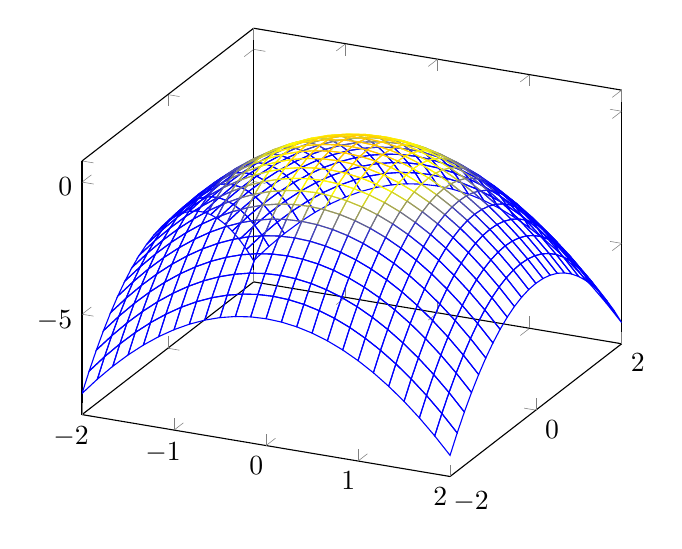
\begin{tikzpicture}
        \begin{axis}[samples=25]
        \addplot3[surf,mesh, point meta min=-2, point meta max=2, domain=-2:2] {-x^2-y^2};
        \end{axis}
        \end{tikzpicture}}
        \\
        \scalebox{0.69}{
        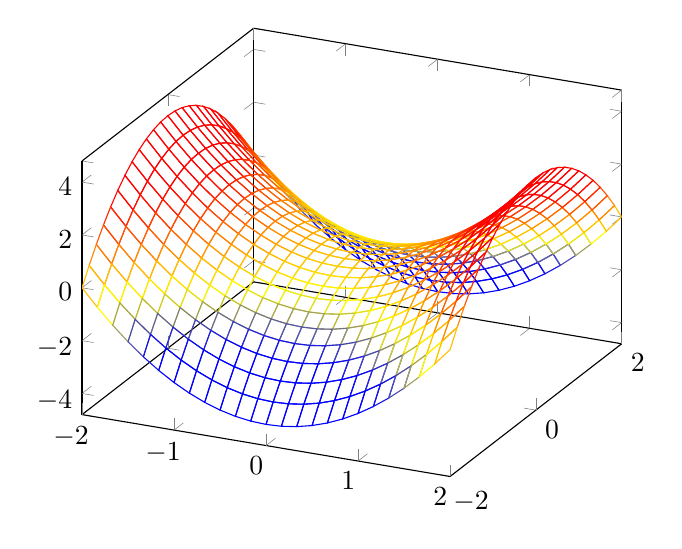
\begin{tikzpicture}
        \begin{axis}[samples=25]
        \addplot3[surf,mesh, point meta min=-2, point meta max=2, domain=-2:2] {x^2-y^2};
        \end{axis}
        \end{tikzpicture}}
        \\
        \scalebox{0.69}{
        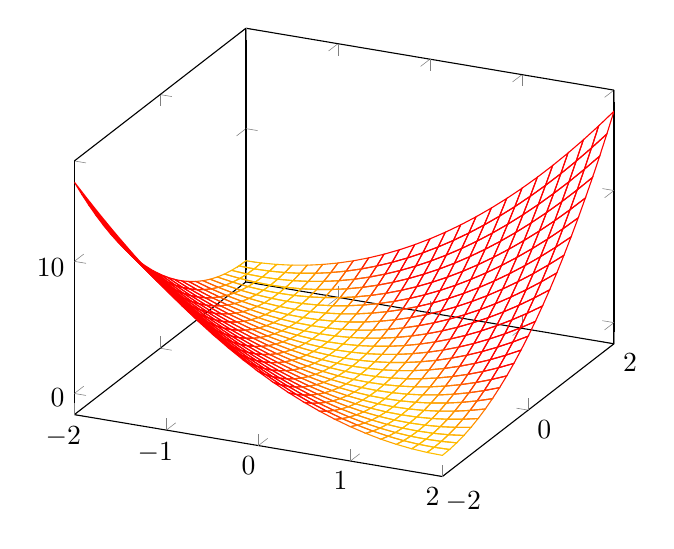
\begin{tikzpicture}
        \begin{axis}[samples=25]
        \addplot3[surf,mesh, point meta min=-2, point meta max=2, domain=-2:2] {x^2+2*x*y+y^2};
        \end{axis}
        \end{tikzpicture}
        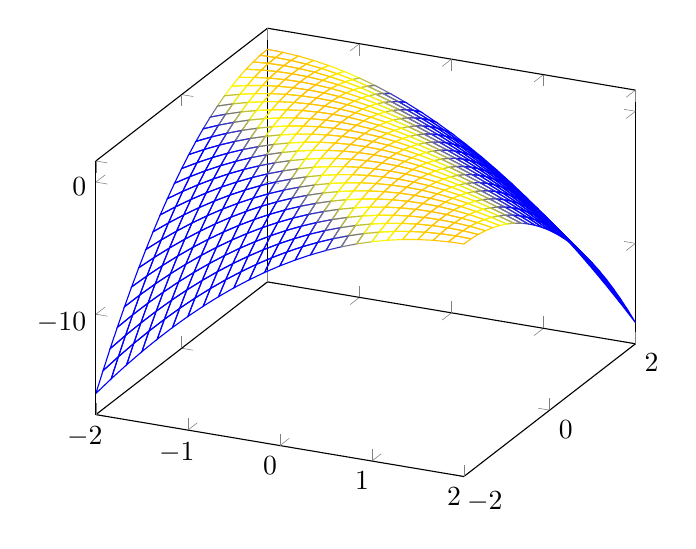
\begin{tikzpicture}
        \begin{axis}[samples=25]
        \addplot3[surf,mesh, point meta min=-2, point meta max=2, domain=-2:2] {-x^2-2*x*y-y^2};
        \end{axis}
        \end{tikzpicture}
      }
    \end{center}
    \item Forms of higher degrees are possible, but visualizing surfaces past \(\mathbb{R}^3\) is not really possible here. 
  \end{itemize}
    
\end{itemize}

\newpage
\section{Properties of Quadratic Form}\label{Properties of Quadratic Form}
\begin{itemize}
  \item[]
  
  \subsection{Normalized Quadratic Form}\label{Normalized Quadratic Form}
  \begin{itemize}
    \item Both \(\ttt{\bm{S}}\) and \(\str{\bm{w}}\) help determine the minimization/maximization of the energy of the quadratic form.
    \item Using the geometric examples above, or through analysis of the signs of the coefficients in the polynomial form, then it's clear that finding the min/max is either \(\pm \infty\) or 0.
    \item \dd{Normalized quadratic form}: a normalization of the quadratic form via division of the magnitude of the vector \(\str{\bm{w}}\), i.e.,
    \[%%%%%%%%%%%%%%%%%%%%%%%%%%%%%%%%%%%%%%%%%%%%%%%
    \frac{\str{\bm{w}}^T \ttt{\bm{S}} \str{\bm{w}}}{\str{\bm{w}}^T\str{\bm{w}}}
    \]%%%%%%%%%%%%%%%%%%%%%%%%%%%%%%%%%%%%%%%%%%%%%%%
    \item The normalization provides a useful means for analysis of the energy landscape of the matrix in question by removing trivial changes due to \(\str{\bm{w}}\).
  \end{itemize}

  \subsection{Definiteness}\label{Definiteness}
  \begin{itemize}
    \item \dd{Definiteness}: the reference to the sign of the energy landscape of a square symmetric matrix, with a relationship to the eigenvalues and invertibility of the matrix.
    
    \begin{table}[h]
      \centering
      \begin{tabular}{cm{3cm}cc}
        \toprule
        Category & \centering Geometry  & Eigenvalues & Invertible \\
        \midrule 
         \(\rrr{\underbrace{\textbf{Positive definite}}_{
           \bm{x}^T \bm{S} \bm{x}~>~0~\forall~\bm{x}~\in~\mathbb{R}^n~\setminus~\left\{\bm{o}\right\}
         }}\) &
          \scalebox{0.42}{
          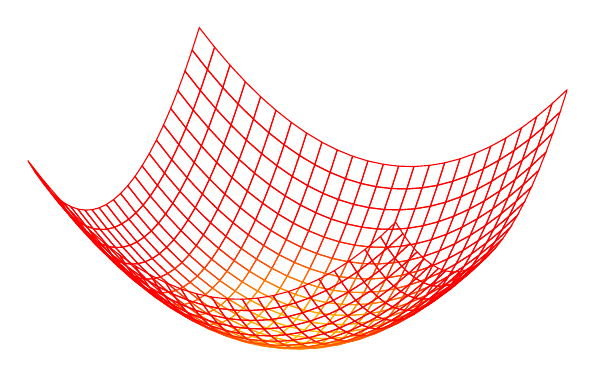
\begin{tikzpicture}
          \begin{axis}[samples=25,hide axis]
          \addplot3[surf,mesh, point meta min=-2, point meta max=2, domain=-2:2] {x^2+y^2};
          \end{axis}
          \end{tikzpicture}}\vspace{3pt} & 
          \rrr{\(+\)} & \true{True}  \\
          \(\str{\underbrace{\textbf{Positive semi-definite}}_{
            \bm{x}^T \bm{S} \bm{x}~\geq~0~\forall~\bm{x}~\in~\mathbb{R}^n
          }}\) &
         \scalebox{0.42}{
          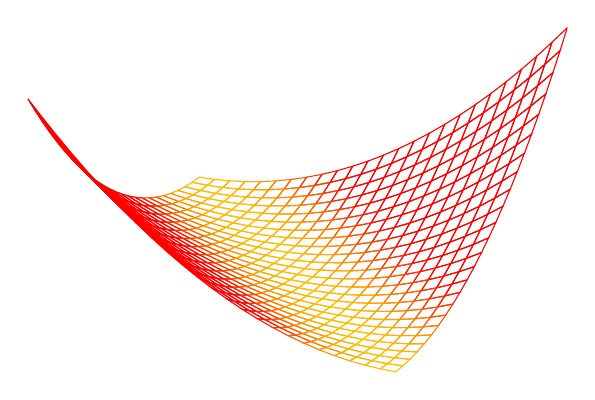
\begin{tikzpicture}
          \begin{axis}[samples=25,hide axis]
          \addplot3[surf,mesh, point meta min=-2, point meta max=2, domain=-2:2] {x^2+2*x*y+y^2};
          \end{axis}
          \end{tikzpicture}}\vspace{3pt} &
          \str{+, 0} & \false{False}  \\
         \textbf{Indefinite} &
         \scalebox{0.42}{
          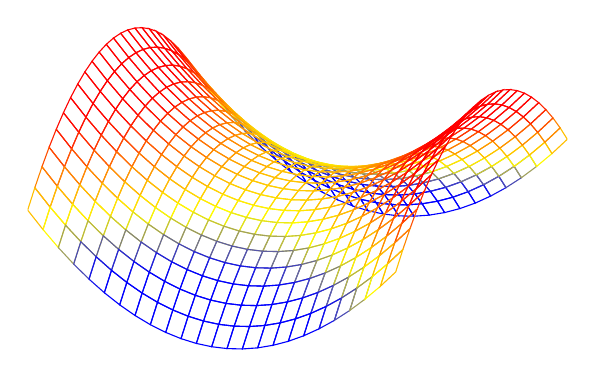
\begin{tikzpicture}
          \begin{axis}[samples=25,hide axis]
          \addplot3[surf,mesh, point meta min=-2, point meta max=2, domain=-2:2] {x^2-y^2};
          \end{axis}
          \end{tikzpicture}}\vspace{3pt} &
         \(\pm\) & \textbf{?} \\
         \(\chap{\underbrace{\textbf{Negtive semi-definite}}_{\bm{x}^T \bm{S} \bm{x}~\leq~0~\forall~\bm{x}~\in~\mathbb{R}^n
          }}\)  &
         \scalebox{0.42}{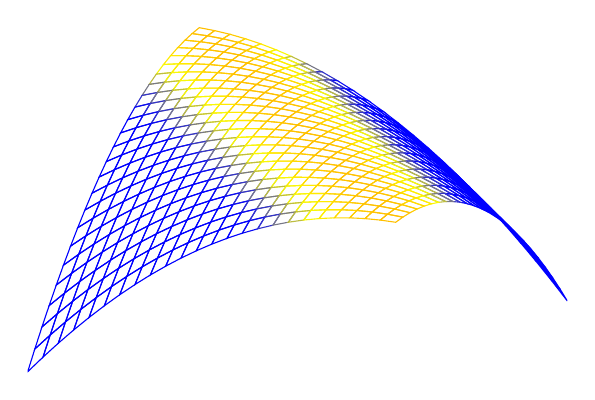
\begin{tikzpicture}
          \begin{axis}[samples=25,hide axis]
          \addplot3[surf,mesh, point meta min=-2, point meta max=2, domain=-2:2] {-x^2-2*x*y-y^2};
          \end{axis}
          \end{tikzpicture}}\vspace{3pt} &
          \chap{\(-,0\)} & \false{False} \\
          \(\bbb{\underbrace{\textbf{Negative definite}}_{
            \bm{x}^T \bm{S} \bm{x}~<~0~\forall~\bm{x}~\in~\mathbb{R}^n~\setminus~\left\{\bm{o}\right\}
          }}\) &
         \scalebox{0.42}{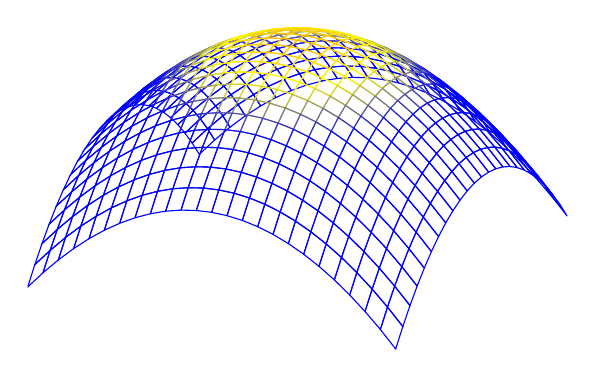
\begin{tikzpicture}
          \begin{axis}[samples=25,hide axis]
          \addplot3[surf,mesh, point meta min=-2, point meta max=2, domain=-2:2] {-x^2-y^2};
          \end{axis}
          \end{tikzpicture}}\vspace{12pt} &
          \bbb{\(-\)} & \true{True} \\ 
          \bottomrule
        \end{tabular}
    \end{table}
    
  \end{itemize}
  
  
  
\end{itemize}


